\chapter{Theoretical Background}

This section introduces existing algorithms, data structures, and metrics relevant to the thesis. First, various types of geometries and common encoding schemes for singular geometries are introduced. Next, descriptions of some compression algorithms in different categories are provided, followed by in-depth details on floating-point representations and delta encoding. Finally, additional compression schemes, some evaluation metrics, and an introduction to spatial indexing are presented. The sections marked with an asterisk (*) are not directly referenced in the thesis and are therefore optional, but may provide a deeper knowledge of existing compression algorithms and understanding of the design choices made in Chapter \ref{sec:chapterimplementation}.

% \todo{\textbf{*}}

\section{Geometries \& Encoding}
\subsection{Geometry Types}
%https://en.wikipedia.org/wiki/Well-known_text_representation_of_geometry
%+ Spatial Parquet paper
\begin{figure}[htbp]
    \centering
    \includesvg[width=8.8cm]{images/geom_types.svg}
    \caption{Descriptions of different geometry types.}
    \label{img:geom_type}
\end{figure}
Four primary types of geometries are commonly used in geometry frameworks: Point, LineString, Polygon, and GeometryCollection. Multipart alternatives consisting of several primitive geometries, such as MultiLineString, are also often included \cite{spatialparquet}.

\begin{description}
    \item[Point] is represented by a pair of the $(x, y)$ coordinates in the plane.
\item[LineString] also referred to as Polyline, is a sequence of points $\langle(x_1,y_1), ..., (x_n,y_n)\rangle$, where two adjacent points in the sequence form a straight line segment.

\item[Polygon] is similar to LineString, but the last point is always equal to the first point, such that the line segments form a closed path. As seen in Figure \ref{img:geom_type}, a polygon may include additional closed paths within the shell, forming holes in the shape. The paths, called \emph{rings}, are represented by a sequence of closed LineStrings, where the first ring is the shell.

\item[GeometryCollection] is a set of geometries, where each geometry can be of any type supported by the framework, including another GeometryCollection. The collections can therefore be used to categorize shapes into a tree-like structure.
\end{description}

Furthermore, as seen in Figure \ref{img:geom_type}, shapes may consist of multiple combined geometries of the same type, namely MultiPoint, MultiLineString, and MultiPolygon. The approach for storing those geometries is similar to GeometryCollection, but without recursive types \cite{spatialparquet}.


\subsection{Geometry Encoding}
% \todo{side by side}

\begin{figure}[htbp]
    \centering
\begin{lstlisting}[language=json,firstnumber=1,basicstyle=\footnotesize\ttfamily]
{ "type": "FeatureCollection",
  "features": [
  {   "type": "Feature",
      "geometry": {
        "type": "Point"
        "coordinates": [55.2517, 12.6543]},
      "properties": { "map_type": "POI" }
}]}
\end{lstlisting}
\caption{GeoJSON format representing a point.}
    \label{fig:geojson}
\end{figure}



Three commonly used data formats for storing geometries are \textit{well-known text} (WKT), \textit{well-known binary} (WKB), and \textit{GeoJSON}. GeoJSON stores geometry information in a JavaScript Object file, with the geometries starting in a collection called \textit{FeatureCollection}, as shown in Figure \ref{fig:geojson}. For each feature, the type of geometry is indicated in the \textit{type} field, along with additional attributes such as \textit{coordinates} \cite{GeoJSON}.

\begin{figure}[htbp]
\begin{lstlisting}[language=json,firstnumber=1, basicstyle=\footnotesize\ttfamily]
GEOMETRYCOLLECTION (POINT(1.25 3.47), LINESTRING(8.2 2.3, 5.5 1.8))
POINT (2.2 88.1)
POLYGON ((10 60, 70 30, 20 20, 10 20, -30 -10))
\end{lstlisting}    
\caption{Well-known text (WKT) format representing a GeometryCollection, LineString, Point, and Polygon.}
    \label{fig:wkt}
\end{figure}

The more straightforward WKT format, as seen in the example in Figure \ref{fig:wkt}, represents each geometry in plain text with the geometry type followed by an ordered sequence of coordinates. The ordered sequence of coordinates can be divided into groups, notated by encapsulating parenthesis, to maintain the geometry structures. For instance, in a polygon with holes, each ring's coordinates are held within separate parenthesis \cite{WKT}.

Well-known binary is information-wise equivalent to well-known text, but it is represented in a more compact binary form and is better served for data transportation \cite{WKB}. Even though these three geometry representations vary in size, they are all considered to be in uncompressed form.





%https://en.wikipedia.org/wiki/Well-known_text_representation_of_geometry
%https://en.wikipedia.org/wiki/GeoJSON#Example
%https://en.wikipedia.org/wiki/OpenStreetMap
%https://medium.com/@thegeospatialnews/how-are-google-maps-different-from-openstreetmap-bc65f704cdab

\section{Introduction to Compression}
The following section explains some of the principle concepts used in compression, while Table \ref{table:compalgos} provides a brief overview of some of the most commonly used compression schemes. 

%https://geekyhumans.com/de/most-popular-data-compression-algorithms/
%https://en.wikipedia.org/wiki/Data_compression
%https://ethw.org/History_of_Lossless_Data_Compression_Algorithms
%https://www.researchgate.net/publication/317599235_Modern_Lossless_Compression_Techniques_Review_Comparison_and_Analysis

% \todo{NOTE: Jag har gjort lite ändringar i tabellen så kopiera in den om du gör ändringar så det inte skrivs över}



\subsection{Lossy and Lossless Methods}
Compression algorithms can be divided into two categories; lossy and lossless methods. Lossless methods allow for the compressed data to be fully restored by decompression. In contrast, lossy methods allow some data to be permanently lost to achieve a higher compression ratio. 

Lossless methods are usually purely algorithmic, focusing on structuring the data in a clever way such that the algorithm can be performed backwards to restore the data back to its original form.

On the other hand, lossy methods are often statistically based, where an approximative model is created, which can be used to predict the original data based on features and context. For example, neighboring pixels in an image are likely to be similar in color. By accepting some, often indistinguishable, loss, a higher compression ratio can be achieved since small variations in the data can be ignored. Furthermore, domain-specific optimizations, such as removing frequencies that are out of the human hearing range and reducing the color palette in images, are considered lossy methods. 

Some areas which use lossless methods are scientific research data, general file compression algorithms (ZIP, RAW, FLAC), and databases. Lossy compression is used in, for example, 
images and video, voice communication, and audio files (MP3) \cite{lossyAndLossless}.

\begin{table}[H]
{\setlength{\extrarowheight}{9pt}%

\resizebox{\textwidth}{!}{%
\begin{tabular}{|l|l|l|l|}
\hline
\textbf{Is Lossless} & \textbf{Compression Type} & \textbf{Algorithm} & \textbf{Description} \\ \hline
\multirow{19}{*}{Yes} & \multirow{6}{*}{Dictionary-based} & LZ77 & Sliding window to find repeated patterns \\ \cline{3-4} 
 &  & LZ78 & LZ77 with dynamic dictionary \\ \cline{3-4} 
 &  & LZMA & LZ77 with range coding \\ \cline{3-4} 
 &  & LZMA2 & LZMA with chunking for multithreading \\ \cline{3-4} 
 &  & LZW & Faster version of LZ78 \\ \cline{3-4}
 &  & LZS & LZ77 with sliding window and stack \\ \cline{2-4} 
 & \multirow{6}{*}{Entropy-based} & Deflate & LZ77 followed by Huffman coding \\ \cline{3-4} 
 &  & bzip2 & Several stacked compression techniques.\\ \cline{3-4} 
 &  & Huffman coding & Encode common values with fewer bits \\ \cline{3-4} 
 &  & ZStandard & Deflate with improved speed \\ \cline{3-4} 
 &  & Arithmetic coding & Fractional encoding of symbol sequences \\ \cline{2-4} 
 & \multirow{3}{*}{Statistical Modelling} & PPM & Context modelling and prediction \\ \cline{3-4} 
 &  & Sequitur & Uses a context-free grammar to encode repetitions \\ \cline{3-4} 
 &  & Re-Pair & Recursively constructs a context-free grammar \\ \cline{2-4} 
 & \multirow{4}{*}{Transform-Based} & DCT & Transform to frequency domain \\ \cline{3-4} 
 &  & Burrows-Wheeler & Rearranging symbol in a reversible manner \\ \cline{3-4} 
 &  & Move to front & Rearranging symbols based on their frequency. \\ \cline{2-4} 
 & \multirow{2}{*}{Other} & RLE & Remove sequential repetition \\ \cline{3-4} 
 &  & Delta encoding & Store value differences \\ \hline
\multirow{2}{*}{Both} & \multirow{2}{*}{NN-based} & MLP & Compression using Multi Layer Perception \\ \cline{3-4} 
 &  & CNN & Compression by Convolutional Neural Networks \\ \hline
\multirow{4}{*}{No} & \multirow{2}{*}{Transform-based} & JPEG & Discard unnoticeable differences in images \\ \cline{3-4} 
 &  & MPEG & Discards unnoticeable differences in video \\ \cline{2-4} 
 & \multirow{2}{*}{NN-based} & GAN & Compression by Generative Adversarial Networks \\ \cline{3-4} 
 &  & Deep Coder & Code compression by Neural Network techniques \\ \hline
\end{tabular}%
}}
\caption{Descriptions of common compression schemes divided into various categories.}
\label{table:compalgos}
\end{table}

\subsection{Entropy Encoding}
In information theory, the entropy quantifies the expected number of bits required to hold the information in a sequence of symbols \(H(X)\) with the formula: 
\begin{equation}
    H(X) = - \sum_{x}  P(x) \cdot \log_2(P(x))
    \label{eq:entropy}
\end{equation} where $X$ is a random variable on the symbols and \(P(x)\) is the probability of a symbol \(x\). The insight behind it is that more predictable information requires less storage on average, and for symbols with a probability distribution, each character has a predictable code length. Accordingly, 
\textit{Shannon's Source Coding Theorem} states that the entropy provides a lower bound for the average number of bits required to represent a discrete sequence of symbols, denoted as \(C\)  \cite{shannon}.
\begin{equation}
   H(X) \leq C
    \label{eq:entropyoptimal}
\end{equation} Additionally, an assumption for the theorem is that the symbols in the discrete sequence are independent and identically distributed.

Entropy encoding is a lossless compression scheme that utilizes this insight, and each symbol in the input is assigned a particular variable-length prefix code according to its probability. In other words, frequent symbols are encoded with fewer bits than infrequent ones. The most common entropy encoding schemes are arithmetic encoding and Huffman encoding \cite{Entropy2, entropyEncoding}.

\subsection{Local Decompression}

Local decompression refers to the action of only decompressing a fraction of the data. A prerequisite for local decompression is the ability to query for specific parts of the data and, in turn, specify and extract only the necessary sections for decompression \cite{localDecomp}.

The advantages of local decompression become evident when performing operations on compressed data, as such operations often experience delays caused by the overhead of making the data operationally available through decompression. One way to reduce the unnecessary overhead is by pre-computing the operation's result and storing it separately from the compressed data. However, this is only beneficial when the operation adds only an insignificant amount of data. For operations resulting in large-size data, local decompression followed by executing the operation may be better suited. With this approach, the delay is shortened by only decompressing the sections necessary for the operation. 

Another use case for local decompression is allowing random access on compressed data, where only some indexable parts of the uncompressed data are accessed. Random access can be implemented by applying local decompression on indexed data fragments.


\section{Delta Encoding}
% \todo{fixa topic sentences}

\subsection{Zigzag Encoding}
Zigzag encoding is a transformation of two's complement such that the positive and negative representation of a value share initial symbols. The transformation ensures that small magnitude numbers, regardless of their signedness, have leading zeros. In contrast to two's complement, where the most significant bit represents signedness, Zigzag encoding uses the least significant bit instead. Following that, the integer's absolute value is shifted one position to the left \cite{zigzagencoding}. The encoding is particularly useful when dealing with negative integers of small magnitude, as evident by the 16-bit example given in Equation \ref{eq:zigzag}. 
\begin{equation}
-5_{dec} = 1111\ 1111\ 1111\ 1011_{two's} = 0000\ 0000\ 0000\ 1011_{zigzag}
\label{eq:zigzag}
\end{equation}

Functions for converting between zigzag and two's complement representation using two's complement arithmetic are given by Equation \ref{eq:zigencode} and Equation \ref{eq:zigdecode} \cite{zigzagencoding}:
\begin{equation}
zigzag\_encode(n)= \begin{cases}2 n, & \text { if } n \geq 0 \\ 2 |n|-1, & \text { if } n<0\end{cases}
\label{eq:zigencode}
\end{equation}

\begin{equation}
zigzag\_decode(n) = \begin{cases}\frac{n}{2}, & \text { if } n \text { even } \\ -\frac{n+1}{2}, & \text { if } n \text{ odd } \end{cases}
\label{eq:zigdecode}
\end{equation}


%https://unbscholar.lib.unb.ca/islandora/object/unbscholar%3A9399/datastream/PDF/view
\label{section:fpd}
\subsection{Integer Delta Encoding}
One way to reduce the file size of integer data is by using delta encoding, which encodes the differences between consecutive numbers instead of the absolute values. This approach can be effective because the bit-length of an integer is directly proportional to its value, so reducing the value can lead to a reduction in the number of required bits. Delta encoding can achieve a high compression ratio when consecutive integers are close in value and a compression technique for small integers is used \cite{intcomp}.

Variable-Byte encoding is one example of a coding technique that compresses small integers effectively. This technique works by reserving one bit in each byte to indicate whether the current byte is the last byte in the integer. By using this method when the most significant bytes in an integer contain all zeros, the encoder can eliminate some of the leading zeros, which can significantly reduce its size \cite{intcomp}.

\subsection{Floating-Point Delta Encoding}
\label{section:fpd_enc}
\begin{figure}[H]
    \centering
    \includesvg[width=12.5cm]{images/float32.svg}
    \caption{The representation of a float32, according to the IEEE 754 binary32 standard. The IEEE 754 binary64 (double64) is analogous, with the exponent being 11 bits, and the mantissa being 52 bits.}
    \label{img:f32}
\end{figure}

When dealing with geometries, floating-point numbers are frequently used instead of integers. Unlike integers, a smaller floating-point magnitude does not mean that the representation uses fewer bits. The most commonly used floating-point standard is IEEE 754, and as illustrated in Figure \ref{img:f32}, it consists of three parts: the sign, exponent, and mantissa \cite{fpbasics}. The mantissa holds the fractional part and contributes to the precision, while the exponent scales the value of the mantissa and determines the position of the decimal point. To convert a binary32 representation to its decimal value, the formula in Equation \ref{fpeq} can be used.

\begin{equation}
V_{dec} = (-1)^S \cdot 2^{E-127} \cdot (1 + \frac{M}{2^{23}})
\label{fpeq}
\end{equation}

Floating-point delta encoding is a technique that exploits the fact that two points in proximity tend to have the same or similar sign and exponents in their coordinates \cite{spatialparquet}. Moreover, if the exponents are equal, the fractions are also likely to be close in value. To calculate the FP-delta encoding, two consecutive floating-points' IEEE 754 representations are interpreted as integers, and their difference is calculated. If the sign and exponents are the same, they cancel each other, leaving the difference between the fractions. Zigzag encoding can then be applied to map negative deltas to positives, resulting in a representation with leading zeros.

When the encoding is initialized, the encoder outputs the initial value and the bit count \(n^*\), which indicates how many bits are used to encode each delta. Subsequent values are then processed until encountering a delta that cannot be represented by \(n^*\) bits. When this occurs, a reset marker consisting of the highest possible zigzag-delta value is output, and the encoding process restarts from the new value. Furthermore, the thesis significantly uses the concept of \textit{chunks}. In this context, a \textit{chunk} is defined as the sequence from the reset point to the last local delta. Thus, the FP-delta encoding consists of one or multiple chunks, depending on the values of the deltas. 

The value of \(n^*\) is, consequently, a trade-off between the number of bits per delta and the number of delta overflows, which requires the encoder to output the reset marker and initial value again. \citet{spatialparquet} presents a method for calculating an optimal \(n^*\) by scanning the entire dataset and logging the number of bits required to encode each delta. With this approach, it is also possible to calculate the final compressed size to determine whether the use of delta encoding is worthwhile or not.

\subsection{An Example of Floating-Point Delta Encoding}
This section provides an illustration of the process and potential benefits of FP-delta encoding a sequence of points. To demonstrate the process, a sequence of three points, coded with 64-bit double precision, is randomly selected from the OSM dataset \cite{osmabout}. Since the x- and y-values are typically unrelated, the pairs are encoded separately. For the demonstration, 64-bit floating-points are used, but the process is analogical for 32-bit floating-points.

As described above, one way to indicate the end of a chunk is to use a reset marker. However, for this example, an alternative approach is used in which each chunk header contains the number of deltas within the chunk. This approach is better suited for local decompression, as further explained in the implementation part of the report. Only the x-axis is encoded in the example, and the coordinates are 
listed in Equation \ref{eq:fpcoords}:
\definecolor{numberemph}{RGB}{100, 0, 0}
\begin{equation}
(x_0^{(dec)}, x_1^{(dec)}, x_2^{(dec)}) = (\textcolor{red}{13.202}\textcolor{black}{7968}, \textcolor{red}{13.202}\textcolor{black}{9830}, \textcolor{red}{13.202}\textcolor{black}{7077})
\label{eq:fpcoords}
\end{equation}

The objective is to calculate the floating-point delta representation of the coordinate sequence using the encoding function in Equation \ref{eq:fpddef}. The encoding consists of the sequential sum of all chunks, where each chunk includes the delta count, reset point, and an arbitrary number of deltas, as shown below:
\begin{equation}
    f\hspace{-0.15em}pd([x_0,\ \ldots,\ x_n]) = \sum_{c \in C} \left[m_c,\ x_c,\ \sum_{i=c}^{i = c + m_c} [d_{i,\ i+1}^{(zigzag)}] \right]
\label{eq:fpddef}
\end{equation}
where $C$ is the sequence of index offsets for all chunks, and $m_c$ is the number of deltas within chunk $c$.

The next step is to find the zigzag encoded representation of the deltas $d^{(zigzag)}$, along with $n^*$ to determine the chunk borders. To calculate the optimal \(n^*\), the data is iterated over once while storing the properties for the deltas. More precisely, for all coordinates, the integer representation difference between the current and previous coordinate is calculated, and the number of bits required to represent the difference is noted as a histogram function \cite{spatialparquet}.

Let $D$ be the set of all zigzag encoded deltas in the dataset. The histogram function $h[i]$ can be defined using the $len$-function, which returns the number of bits required to represent a zigzag encoded delta, as shown below in Equation \ref{eq:fphistdef};
\begin{equation}\label{eq:fphistdef}
  \begin{gathered}
    len(d) = \left \lceil{\log_2{(d + 1)}}\right \rceil \\
h[i] = |\ { d \in D : i = len(d) }\ |
  \end{gathered}
\end{equation}

Using the histogram function, it is possible to calculate the resulting size (excluding the first point) for the different \(n\) (Equation \ref{eq:fpsizebit}):
\begin{equation}
S(n)=\underbrace{(b_r+64) \cdot \sum_{i=n+1}^{i=64} h[i]}_{\text{reset points}} + \underbrace{n \cdot \sum_{i=0}^{i=n} h[i]}_{\text{deltas}}
\label{eq:fpsizebit}
\end{equation}

where $b_r$ is the bit-length of the header for the chunk. In this example, the $b_r$ bits are used to store the count of deltas which are part of the next sequence.
\\\\
Using Equation \ref{eq:fpoptn}, $n^*$, which is the optimal $n$ such that $S(n)$ is minimized, is obtained:

\begin{equation}
    n^*={\operatorname{arg\,min}}\{S(n)\}
\label{eq:fpoptn}
\end{equation}
\\\\
To calculate the deltas, the coordinates are interpreted as integers. If 64-bit floating-points are used, the x-values are interpreted according to Equation \ref{eq:fpintrep}:
\begin{equation}
\begin{gathered}
    d_{01}^{(two's)} = x_1^{(int)} - x_0^{(int)} = 4623622236719630774\\ -\ 4623622131898349447 = 104821280768
\end{gathered}
\label{eq:fpintrep}
\end{equation}

Next, the delta values are zigzag encoded using the function in Equation \ref{eq:zigencode}, resulting in Equation \ref{eq:fpzigzagen}:
\begin{equation}
    \begin{gathered}
     d_{01}^{(two's)} \xrightarrow{zigzag\ encode} d_{01}^{(zigzag)} \iff d_{01}^{(zigzag)} = \begin{cases}2 \cdot d_{01}^{(two's)}, & \text { if } d_{01}^{(two's)} \geq 0 \\ 2 \cdot |d_{01}^{(two's)}|-1, & \text { if } d_{01}^{(two's)}<0\end{cases} \\
    d_{01}^{(zigzag)} = 2 \cdot d_{01}^{(two's)} = 209642561536
    \end{gathered}
    \label{eq:fpzigzagen}
\end{equation}


Or equivalently, in binary representation:

\resizebox{14.3cm}{!}{%
\begin{minipage}{14.3cm}
\begin{alignat*}{4}
    &x_1^{(int)}& &=&\ &01000000\ 00101010\ 01100111\ 11101101\ 01100011\ 01000101\ 01001001\ 10110110
&\\   
    -\hspace*{.5em}&x_0^{(int)}& &=&\ &01000000\ 00101010\ 01100111\ 11010100\ 11111011\ 01101111\ 01110111\ 10000111&\\[-2.5ex]\cline{2-8}\\[-4.8ex]
    &d_{01}^{(two's)}& &=&\ &00000000\ 00000000\ 00000000\ 00011000\ 01100111\ 11010101\ 11010000\ 00000000&\\
    &d_{01}^{(zigzag)}& &=&\ &00000000\ 00000000\ 00000000\ 00\underbrace{110000\ 11001111\ 10101011\ 10100000\ 00000000}_{38 \text{ bits}}&
\end{alignat*}
\end{minipage}
}

For $d_{12}^{(two's)}$, in binary representation:

\resizebox{14.3cm}{!}{%
\begin{minipage}{14.3cm}
\begin{alignat*}{4}
    &x_2^{(int)}& &=&\ &01000000\ 00101010\ 01100111\ 11001001\ 01001101\ 10111100\ 01001011\ 01110101&\\   
    -\hspace*{.5em}&x_1^{(int)}& &=&\ &01000000\ 00101010\ 01100111\ 11101101\ 01100011\ 01000101\ 01001001\ 10110110&\\[-2.5ex]\cline{2-8}\\[-4.8ex]
    &d_{12}^{(two's)}& &=&\ &11111111\ 11111111\ 11111111\ 11011011\ 11101010\ 01110111\ 00000100\ 00000000&\\
    &d_{12}^{(zigzag)}& &=&\ &00000000\ 00000000\ 00000000\ 0\underbrace{1001000\ 00101011\ 00010001\ 11111000\ 00000000}_{39 \text{ bits}}&
\end{alignat*}
\end{minipage}
}


Using the resulting delta values from above, $h[i]$ is defined according to Equation \ref{eq:fphistres}:
\begin{equation}
h[i] = \begin{cases}1, & \text{if } i = 38 \text{ or } i = 39 \\ 0, & \text{otherwise} \end{cases}
\label{eq:fphistres}
\end{equation}

The values for $S(n)$ are calculated for $n \in \mathbb{Z} : h[n] \neq 0 $ and the endpoints, as shown in Equation \ref{eq:fpscalc}:
\begin{equation}\label{eq:fpscalc}
  \begin{gathered}
    S(0) = (b_r + 64) \cdot 2 + 0 = 128 + 2b_r \\
    S(38) = (b_r + 64) \cdot 1 + 38 \cdot 1  = 102 + b_r \\
    S(39) = 0 + 39 \cdot 2= 78 \\
    S(64) = 0 + 64 \cdot 2 = 128
  \end{gathered}
\end{equation}

The values in Equation \ref{eq:fpscalc} show that using 39 bits to encode the deltas will result in a total size of $(b_r + 64) + 78 = 142 + b_r$ bits. Here, the first $b_r + 64$ bits correspond to the first point (which cannot be delta encoded) and the initial chunk header. Assuming that $b_r$ is chosen optimally in terms of size, this results in a smaller total size than the uncompressed $64 \cdot 3 = 192$ bits.

Once $n^*$ has been found, the resulting output stream can be generated by enumerating the deltas. If a delta fits within the $n^*$ bits, it is directly output. Otherwise, a reset point consisting of the delta count and coordinate is output. With $n^*=39$, the resulting output stream is as expressed in Equation \ref{eq:fpdresult}:
\begin{equation}
    f\hspace{-0.15em}pd([x_0,\ x_1,\ x_2]) = [2,\ x_0,\ d_{01}^{(zigzag)},\ d_{12}^{(zigzag)}]
    \label{eq:fpdresult}
\end{equation}
where $x_0$ and $d^{(zigzag)}$ are encoded using 64 and 39 bits, respectively. Therefore, for the given example, the smallest size is achieved by using only one chunk.
\\\\
The process of decoding is similar to encoding:
\begin{enumerate}
    \item Load the 64-bit reset point, corresponding to $x_0^{(dec)}$.
    \item Zigzag decode the next delta $d_{01}^{(zigzag)}$, resulting in $d_{01}^{(two's)}$.
    \item Interpret the reset point and the delta as integers, $x_0^{(int)}$.
    \item Add the reset point and delta, $x_1^{(int)} = x_0^{(int)} + d_{01}^{(two's)}$.
    \item Interpret the sum as a 64-bit floating-point value, $x_1^{(dec)}$.
    \item The absolute coordinate $x_1^{(dec)}$ becomes the reset point in (1), and the process is repeated from (2) until all deltas have been processed.
\end{enumerate}

\section{Entropy Encoding Techniques}
\subsection{Huffman Encoding}
\label{section:huff}
\begin{figure}[htbp]
    \centering
    \includesvg[width=7.5cm]{images/Huffman_tree_2.svg}
    \caption{Huffman tree for encoding characters. The numbers represent frequencies for the characters in the leaf nodes or alternatively the combined frequencies of the characters in the subtrees.}
    \label{img:huff}
\end{figure}
Huffman encoding is a form of entropy encoding where the number of bits used to encode an element is inversely proportional to the logarithm of its probability. Frequent elements are thus encoded with fewer bits, resulting in a reduction in size when the encoding benefits are larger than the overhead. An example of a Huffman tree can be seen in Figure \ref{img:huff}.

The methodology used for creating a Huffman binary tree goes as follows \cite{Sharma2010CompressionUH}:

\begin{enumerate}
    \item Count the frequency for each of the elements and add all the elements, with their corresponding frequency to a set \textit{S}.
    \item Create two leaf nodes of the two least frequent elements in \textit{S} and connect them with a new parent node \textit{p} assigned with their joint frequency value.
    \item Remove the two leaf nodes from the set \textit{S} and add \textit{p} to it.
    \item Repeat from (2) until there is only one element left.
    \item Encode the paths down the tree by, from the root, assigning each left step as 0 and right step as 1.
    \item Convert the elements in the input to their corresponding path code in the Huffman tree.
\end{enumerate}

Some characteristics of Huffman encoding are that the tree creation has time complexity $\mathcal{O}(n)$, assuming that the leaf nodes are already sorted by frequency, and that it is a lossless and optimal encoding scheme \cite{Sharma2010CompressionUH}. 




\subsection{Golomb-Rice Encoding}
Golomb-Rice encoding is a parameterized entropy encoding scheme that assumes that small integers are more frequent than large ones. The encoding uses a straightforward method called unary encoding, where a number \(n\) is encoded as $n$ ones followed by one terminating zero. For example, 5 is represented as \(111110\).

When encoding an integer using Golomb-Rice encoding, the first step is to select a parameter \textit{k} and calculate \(m = 2^k\). For the input \textit{n}, the quotient and remainder of \textit{n} divided by \textit{m} are then extracted using Equation \ref{eq:gomb}.

\begin{equation}
q =\lfloor\frac{n}{m}\rfloor\
   \text{ and }
r = n - qm
\label{eq:gomb}
\end{equation}

The next step is to encode the quotient $q$ using unary encoding, the remainder $r$ as an unsigned integer using $\lfloor \log_2(m) \rfloor$ bits, and then concatenate the bit results into a final Golomb-Rice code \cite{rice2}. The scheme is straightforward, but since the result of the encoding is heavily dependent on the parameter \textit{k}, it is essential to select a suitable value. If the data follows a geometric distribution \(P(X = i) = (1 - p)^{i - 1}p\) where \(0 < p \leq 1\), a suitable parameter $k$  can be calculated using the formula in Equation \ref{eq:rice_form}, which only requires the estimated mean value $\mu^*$ of the data \cite{rice}. 
\begin{equation}\label{eq:rice_form}
k^{*}_{geo} = max \left \{ 0, 1 + \left \lfloor log_2\left ( \frac{ln (\theta  - 1)}{ln(\frac{\mu^* }{\mu^* + 1})} \right ) \right \rfloor \right \},  \textup{where }
 \theta = \frac{\sqrt{5} + 1}{2}
\end{equation}

 Golomb-Rice encoding is optimal in the case where the probability \(P(k) = 2^{-k}\) for the parameter $k$.

\starsubsection{Arithmetic Encoding}
Arithmetic encoding is a technique for entropy encoding symbols, considering the probabilities of their occurrence. To do arithmetic encoding, a table of the probabilities of the symbols in the character space is constructed. Each character is then assigned a unique interval with a width equal to its probability; corresponding to the upper left diagram in Figure \ref{img:arith_enco}. 

%Testade att konvertera till svg. BLEV KATASTROF vid vektoriseringen

%https://www.wisdomjobs.com/e-university/multimedia-tutorial-270/arithmetic-coding-12789.html

To encode a sequence, the probability intervals are recursively subdivided in the exact ordering as the sequence to be encoded. For example, in the lower diagram of Figure \ref{img:arith_enco}, the first recursive step assigns the character C to the interval $(0.3, 0.5]$. The algorithm then subdivides and assigns C's interval to all characters again, with an exact fractional width proportional to their probabilities. When the sequence interval has been created, binary search is used to encode the sequence by recording left (0) or right (1) in the search until the binary search falls within the sequence interval \cite{arithmetic_encoding}. Since interval sizes are proportional to their probability of occurrence, common symbols are assigned wider intervals. Fewer binary search partitions are required to fall within a wide sequence interval, and thus words that mostly contain frequent symbols can be stored using fewer bits.

\begin{figure}[htbp]
    \centering
    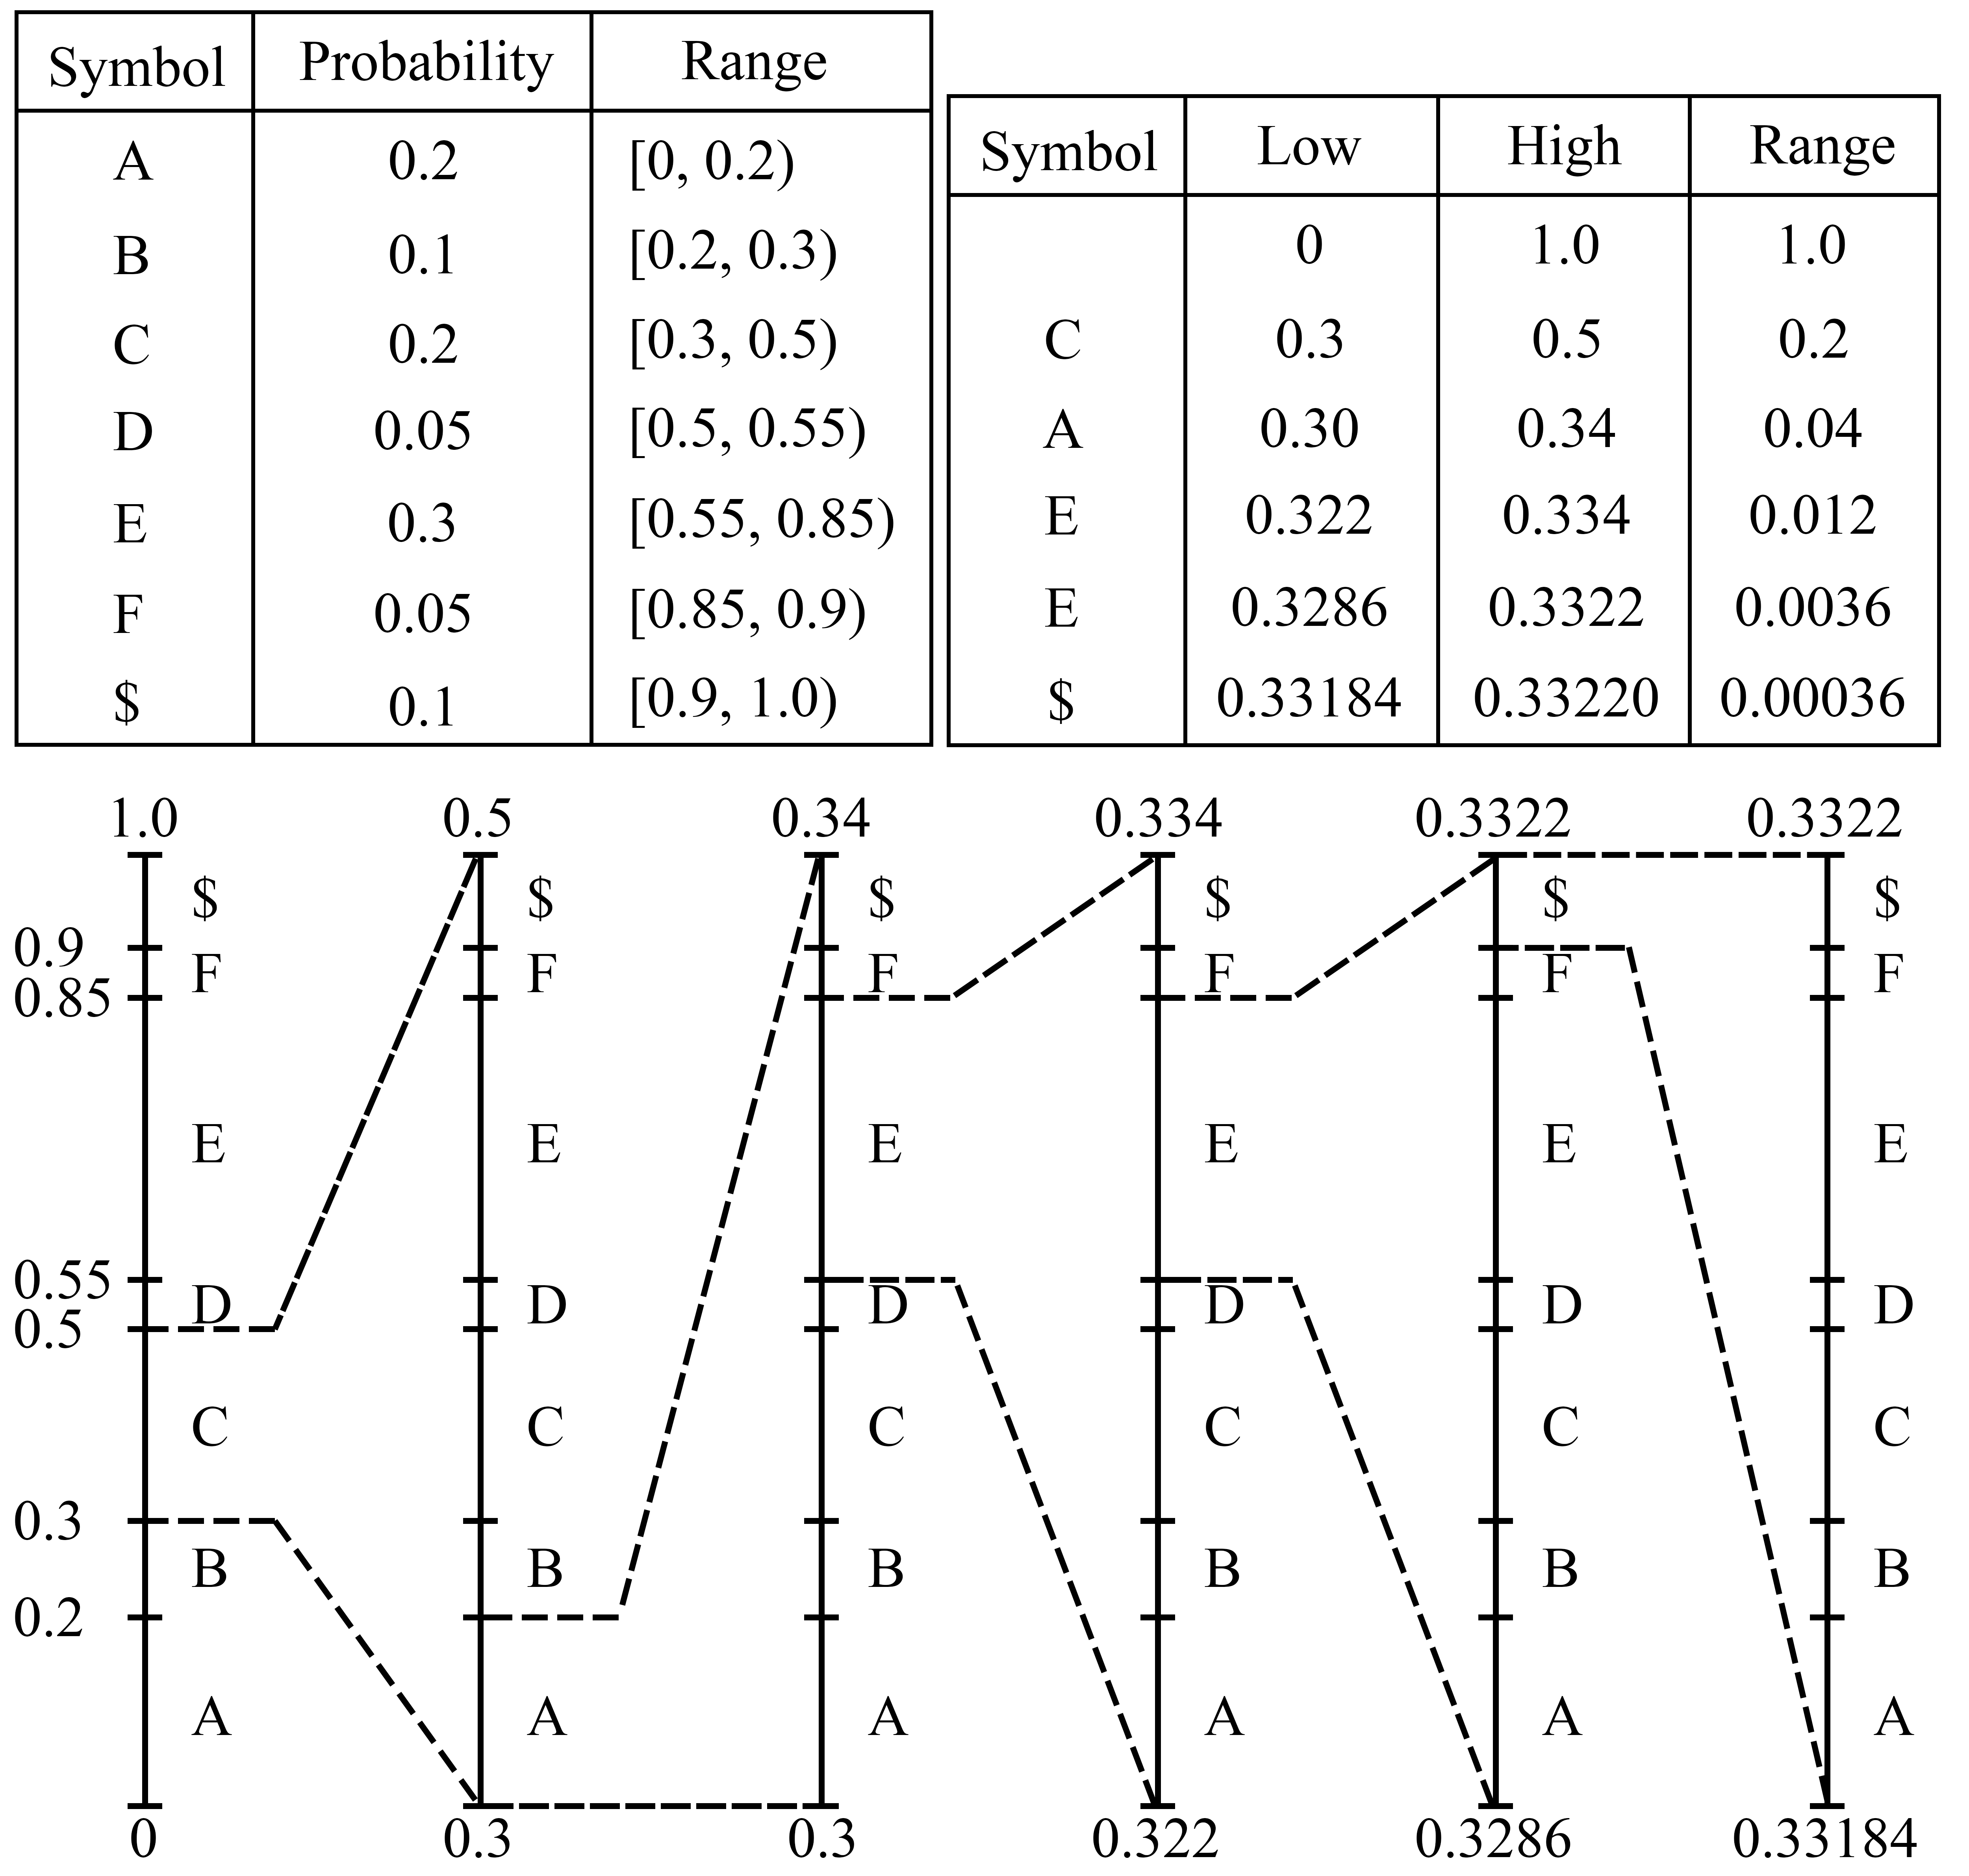
\includegraphics[width=11cm]{images/arithmectic.png}
    \caption{Arithmetic encoding of the character sequence CAEE\$ in the character space ABCDEF\$.}
    \label{img:arith_enco}
\end{figure}


\starsection{Additional Compression Techniques}
\starsubsection{Run-Length Encoding}
Run-Length encoding (RLE) is a lossless encoding scheme that performs well when identical elements frequently appear sequentially. In the sequence AAAABCCCC for example, the characters A and C have adjacent repetitions. Run-Length encoding couples the elements with a number that represents the count of repeated characters. For the example above, the encoding scheme creates the pairs $(\text{A}, 4), (\text{B}, 1), (\text{C}, 4)$ and RLE concatenates the pairs, resulting in an encoding of 4A1B4C.

With its simplicity, RLE provides fast execution, but in most cases RLE results in a lower compression ratio as compared to other algorithms \cite{Sharma2010CompressionUH}. One drawback, as evident by the example above, is that the absence of repetition has to be encoded as well. For text with few repetitions, using RLE will likely increase the size since the gain will be negligible in relation to the overhead. 


\starsubsection{LZ77}
LZ77 is a lossless compression algorithm created by Abraham Lempel and Jacob Ziv in 1977. The intuition behind the algorithm is to remove redundancies of repeated sequences by using pointers to an earlier occurrence of the repetition. 

\begin{figure}[htbp]
    \centering
    \includesvg[width=11cm]{images/lz77.svg}
    \caption{Example of LZ77 encoding of the word sequence \textit{abracadabrad}.}
    \label{img:lz77}
\end{figure}


As illustrated by the example in Figure \ref{img:lz77}, the algorithm uses two sliding windows of predetermined size: a lookahead buffer and a search window. The two windows are aligned, such that the start of the lookahead window is successive to the end of the search window. The idea with the windows is to match the longest sequences in the lookahead buffer, starting at its beginning, with a pointer to the same sequence in the search window. When a match has been found, the two windows shift \(1 + len(match)\) characters along the sequence. A match results in a 3-tuple \textit{(match offset, match length, next nonmatching character)}, which is the output of the algorithm. Decompression is done by performing the process of creating the compressed sequence in reverse \cite{10.1145/356924.356930}. LZ77 is used in current compression algorithms, such as in DEFLATE where it is combined with Huffman encoding. 

\starsubsection{Burrows-Wheeler Transform}
Burrows-Wheeler transform is a method to reorder a string, so the same characters appear sequentially more often. The transformation is invertible, making it possible to go back and forth between the original input string and the transformed version. The invertible property makes it appropriate as a pre-processing step for compression algorithms. For example, Run-Length encoding may perform better when BWT is applied beforehand. To create the Burrows-Wheeler transform, all permutations of the input string, with an inserted marker for the beginning and ending of the string, are generated. The permutations are sorted based on lexical ordering and a sequence containing the last character for each permutation is extracted. As shown in Figure \ref{img:burrow}, the sequence \textit{$\wedge$BANANA $\mid$}, with $\wedge$ and $\mid$ notating the start and end of the sequence, is Burrows-Wheeler transformed into \textit{BNN$\wedge$AA$\mid$A} \cite{Burrows1994ABL}.

\begin{figure}[htbp]
\centering
\resizebox{13cm}{!}{
\begin{tabular}{|lllll|}
\hline
\multicolumn{5}{|c|}{\textbf{Transformation}} \\ \hline
\multicolumn{1}{|c|}{\textbf{Input}} & \multicolumn{1}{c|}{\textbf{All Rotations}} & \multicolumn{1}{c|}{\textbf{Sorting  Rows}} & \multicolumn{1}{c|}{\textbf{Taking Last Column}} & \multicolumn{1}{c|}{\textbf{Output Last Column}} \\ \hline
\multicolumn{1}{|c|}{} & \multicolumn{1}{l|}{\textasciicircum{}BANANA\textcolor{red}{|}} & \multicolumn{1}{l|}{ANANA\textcolor{red}{|}\textasciicircum{}B} & \multicolumn{1}{l|}{ANANA\textcolor{red}{|}\textasciicircum{}\textbf{B}} & \\
\multicolumn{1}{|l|}{} & \multicolumn{1}{l|}{\textcolor{red}{|}\textasciicircum{}BANANA} & \multicolumn{1}{l|}{ANA\textcolor{red}{|}\textasciicircum{}BAN} & \multicolumn{1}{l|}{ANA\textcolor{red}{|}\textasciicircum{}BA\textbf{N}} & \\
\multicolumn{1}{|l|}{} & \multicolumn{1}{l|}{A\textcolor{red}{|}\textasciicircum{}BANAN} & \multicolumn{1}{l|}{A\textcolor{red}{|}\textasciicircum{}BANAN} & \multicolumn{1}{l|}{A\textcolor{red}{|}\textasciicircum{}BANA\textbf{N}} & \\
\multicolumn{1}{|l|}{\textasciicircum{}BANANA\textcolor{red}{|}} & \multicolumn{1}{l|}{NA\textcolor{red}{|}\textasciicircum{}BANA} & \multicolumn{1}{l|}{BANANA\textcolor{red}{|} \textasciicircum{}} & \multicolumn{1}{l|}{BANANA\textcolor{red}{|} \textbf{\textasciicircum{}}} & BNN\textasciicircum{}AA\textcolor{red}{|}A \\
\multicolumn{1}{|l|}{} & \multicolumn{1}{l|}{ANA\textcolor{red}{|}\textasciicircum{}BAN} & \multicolumn{1}{l|}{NANA\textcolor{red}{|}\textasciicircum{}BA} & \multicolumn{1}{l|}{NANA\textcolor{red}{|}\textasciicircum{}B\textbf{A}} & \\
\multicolumn{1}{|l|}{} & \multicolumn{1}{l|}{NANA\textcolor{red}{|}\textasciicircum{}BA} & \multicolumn{1}{l|}{NA\textcolor{red}{|}\textasciicircum{}BANA} & \multicolumn{1}{l|}{NA\textcolor{red}{|}\textasciicircum{}BAN\textbf{A}} & \\
\multicolumn{1}{|l|}{} & \multicolumn{1}{l|}{ANANA\textcolor{red}{|}\textasciicircum{}B} & \multicolumn{1}{l|}{\textasciicircum{}BANANA\textbf{\textcolor{red}{|}}} & \multicolumn{1}{l|}{\textasciicircum{}BANANA\textbf{\textcolor{red}{|}}} & \\
\multicolumn{1}{|l|}{} & \multicolumn{1}{l|}{BANANA\textcolor{red}{|} \textasciicircum{}} & \multicolumn{1}{l|}{\textcolor{red}{|}\textasciicircum{}BANANA} & \multicolumn{1}{l|}{\textcolor{red}{|}\textasciicircum{}BANAN\textbf{A}} & \\ \hline
\end{tabular}}
\caption{Example of Burrows-Wheeler transformation of the sentence \textit{BANANA}.}
    \label{img:burrow}
\end{figure}



\section{Evaluation Metrics}
%https://d1wqtxts1xzle7.cloudfront.net/61774586/Comp_com20200113-81589-6qysrz-libre.pdf?1578974392=&response-content-disposition=inline%3B+filename%3DCOMPARISON_OF_LOSSLESS_DATA_COMPRESSION.pdf&Expires=1676575765&Signature=gBodn-UaNo~-5ZUeGpUiLK66qHtwp1Hw7fLBIJ7LSKGo~40COks2cGmLZdzuRBFDZ1O53ChN8UrCBAwjaz9UqpKodkcPMVgvuYlYsn1mZ6UuF4g4Axpw1fyO5b9YsZGmM-K49J05s88F-WaUtzR0v35MyLW9xl-EQex~Zv1Go9Pcb2v31FYNFfxTPXToR3zZlSACIGXDRm6rVtv3~m9XZTcJPrTCAwbflZPUDWimP5d-oyCiIVFhU5su~-MfKOjk3y0r9huIz-jH~OQu3L~QMBgSH6~3w-aXB8vyXYtjqLil0QuiTaIN64KV7FkPljpMl7k4CXt02uYdu-v0dLSADA__&Key-Pair-Id=APKAJLOHF5GGSLRBV4ZA

The most frequently used evaluation metrics for compression are the \textit{compression ratio} and the \textit{compression factor}, presented in Equation \ref{eq:ratioformula}. The compression ratio describes the output size of a compression algorithm relative to the input data size. For instance, a compression ratio of 0.5 means that the compressed data is 50\% the size of the input. The compression factor is simply the inverse of the compression ratio \cite{metric}. In the industry, it is also common to denote the performance by \(X\):\(1\), where \(X\) is the compression factor \cite{ratioIBM}.

\begin{equation}
    \textrm{\textbf{Compression Ratio}}=\frac{\textrm{1}}
    {\textrm{\textbf{Compression Factor}}}=\frac{\textrm{Size of output stream}}
    {\textrm{Size of input stream}}
    \label{eq:ratioformula}
\end{equation}


Execution time is a metric that is used when evaluating the performance of compression schemes and operations. A problem with simply using the absolute execution time is that it can be influenced by factors that are unrelated to the implementations, such as hardware performance \cite{metric}. To ensure a fair comparison, the relative execution time between different runs under the same circumstances can be compared instead. For this to be reliable, a mean of multiple runs should be considered to filter out noise in the measurements.
Calculating the relative execution time can be done as in Equation \ref{eq:speedformula}.



\begin{equation}
    \textrm{\textbf{Relative Execution Time}}=\frac{\textrm{Time for implementation}}{\textrm{Time for baseline}}
    \label{eq:speedformula}
\end{equation}




\section{Spatial Indexing}
%Indexing generellt: https://medium.com/nerd-for-tech/indexing-data-structures-aa7363693c40
One common challenge when dealing with large amounts of data is efficiently retrieving a subset of the data at an arbitrary location in storage, referred to as \emph{random access} queries. Indexing reduces access time by providing a pointer to the relevant data section based on the input data in the query. Spatial indexing is a subfield that focuses on retrieving data based on a geographic location.
\starsubsection{Quadtrees}
\begin{figure}[h]
    \centering
    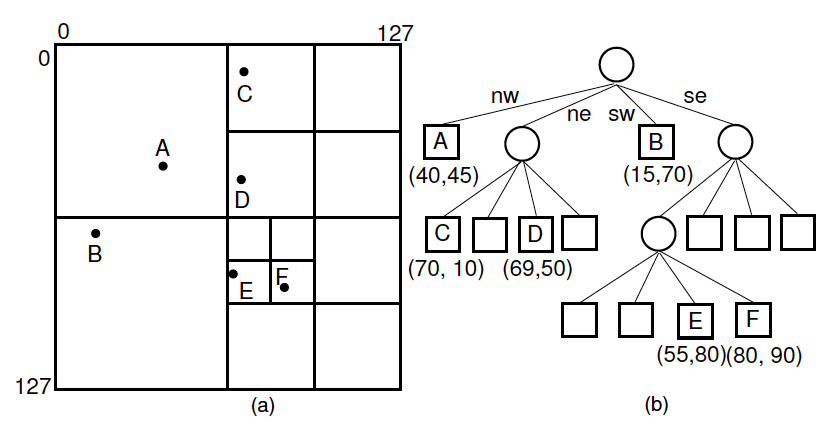
\includegraphics[width=12cm]{images/Point_quadtree.png}
    \caption{An illustration of a quadtree structure in a plane of points. The notation of nw, ne, sw, and se in the tree structure corresponds to the top left, top right, bottom left, and bottom right quadrants, respectively \cite[Figure~13.6]{huffman_tree_img}.} %Same book as huffman img
    \label{img:quad}
\end{figure}
% Riktigt bra sammanfattning av olika indexeringsmetoder
%http://www.cs.siue.edu/~marmcke/docs/cs490/spatialIndexing.html
A quadtree is a hierarchical tree structure where each node has zero or four children. The hierarchical structure enables indexing and makes querying for specific regions of the two-dimensional space convenient.

In a quadtree, each node describes a section of a two-dimensional plane, where the root node describes the section in its entirety. The intuition behind the quadtree is that for a non-leaf node, its four children divide the parent node's two-dimensional section into four quadrants \cite{10.1145/356924.356930}, see Figure \ref{img:quad}.

If a quadrant does not split the data, there is no reason to further divide the section of a node, and it can be assigned as a leaf node. Additionally, the algorithm can stop creating quadrants when a node contains a specified maximum number of data points \cite{10.1145/356924.356930}.

